
A continuacion se discuten los resultados obtenidos por cada dataset
\begin{figure}[H]
    \centering
        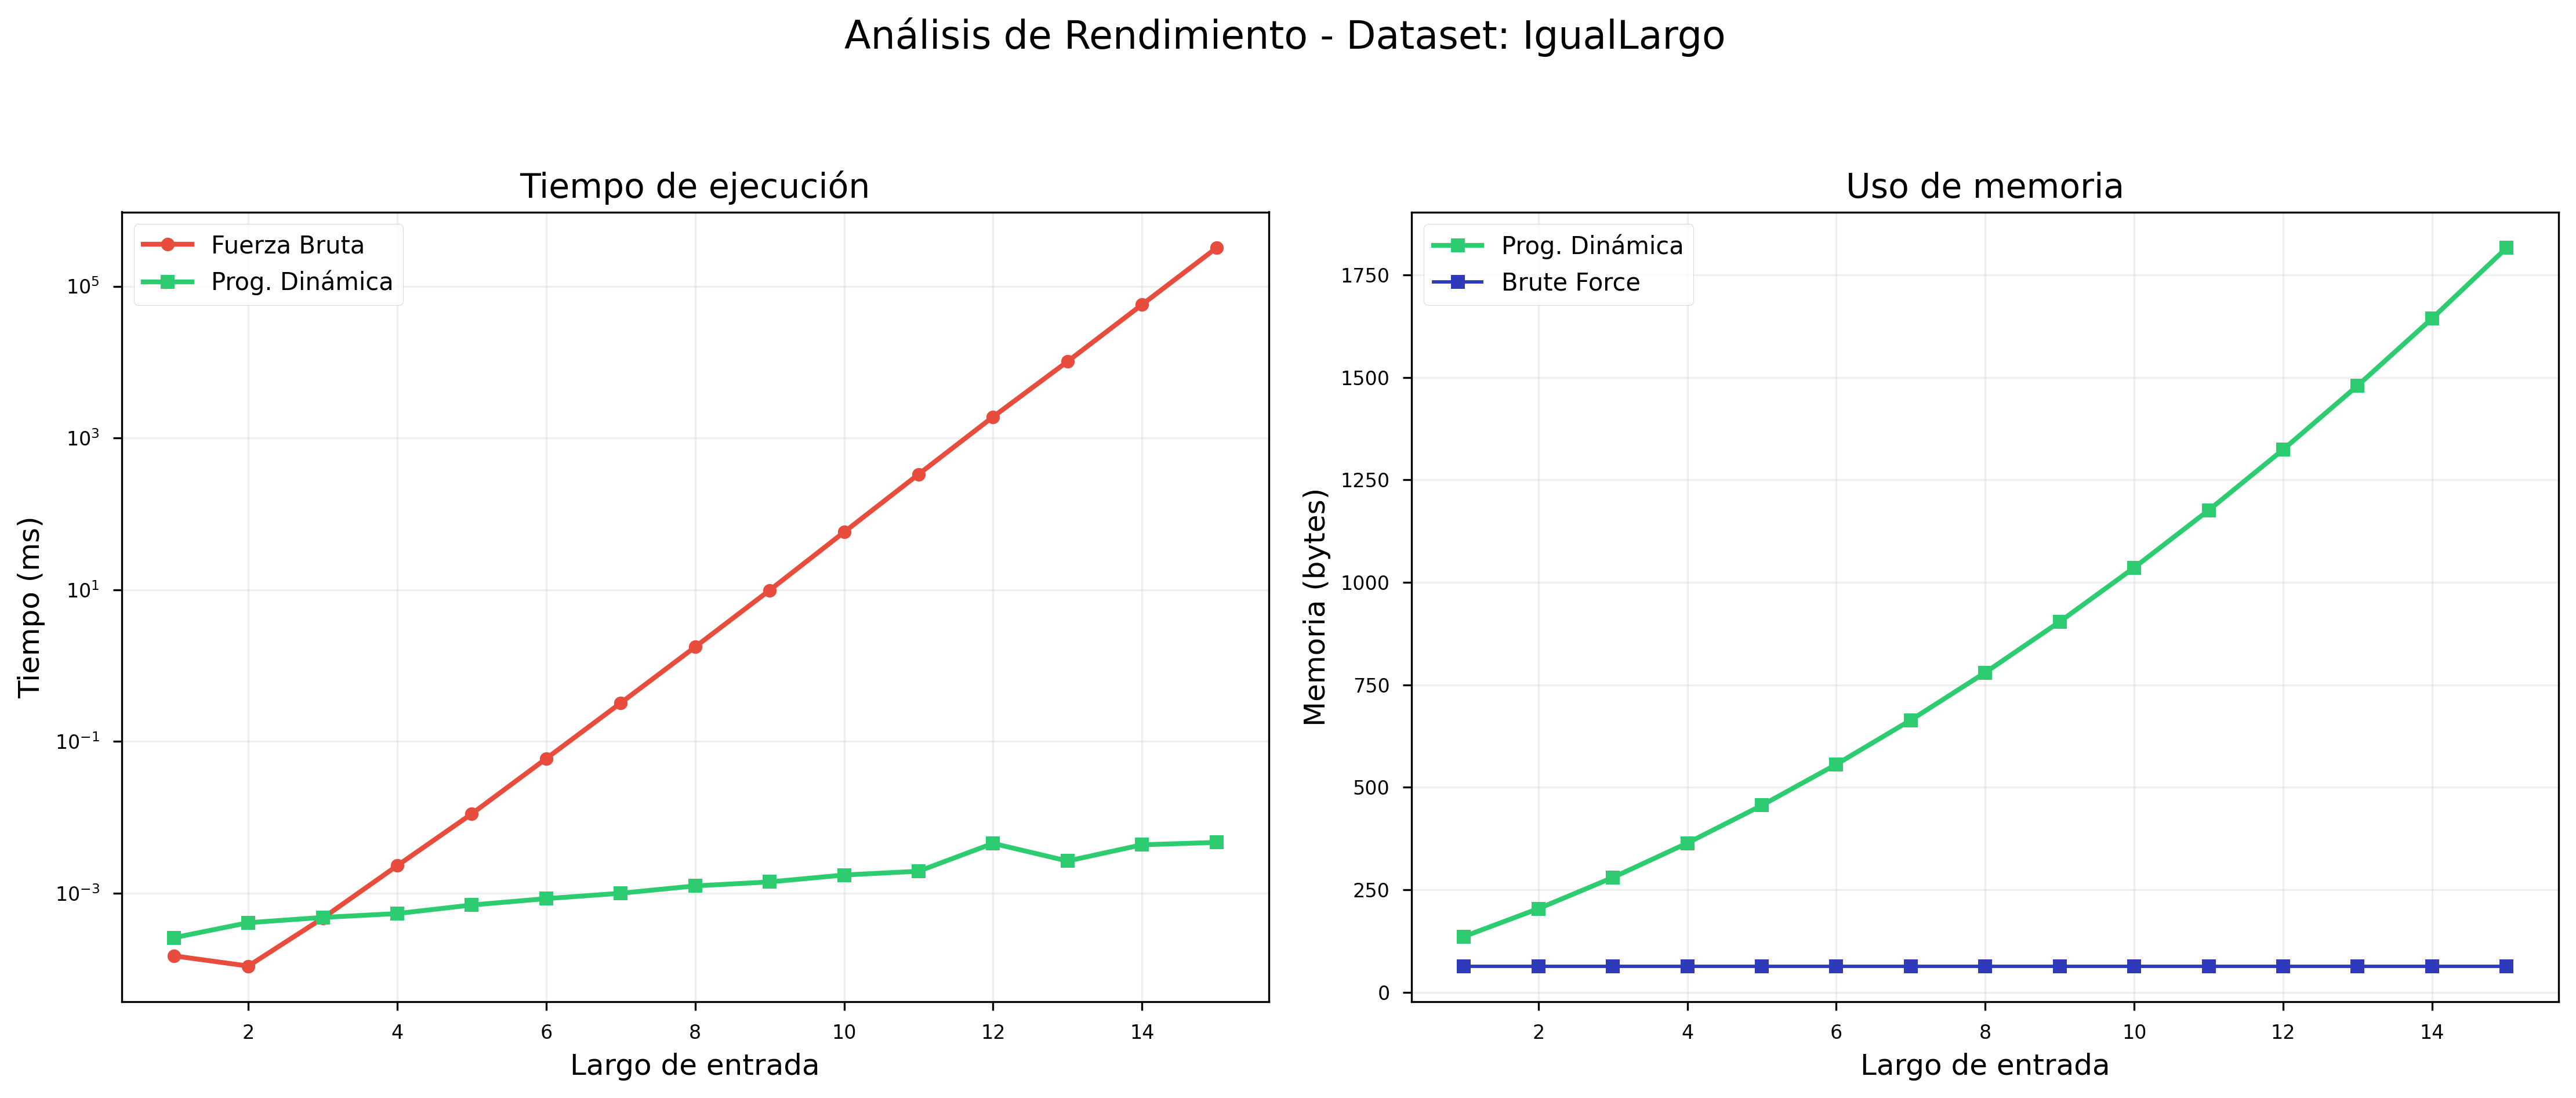
\includegraphics[width=\textwidth]{images/IgualLargo_analisis.png}
    \caption{Cadenas aleatorias de largo creciente}
    \label{fig:scatterplot_1}
\end{figure}
En la figura 1, en el grafico de la iquierda se puede observar la gran diferencia en tiempo de ejecucion de ambos algoritmos a medida que el tamaño
de la entrada crece, aunque la menor complejidad temporal que maneja programacion dinamica es a costa de una mayor complejidad espacial.
El estudio de estos datos es importante puesto que es necesario comprender eperimentalmete que tan sensibles son los algoritmos implementados al tamaño de la entrada

\begin{figure}[H]
    \centering
        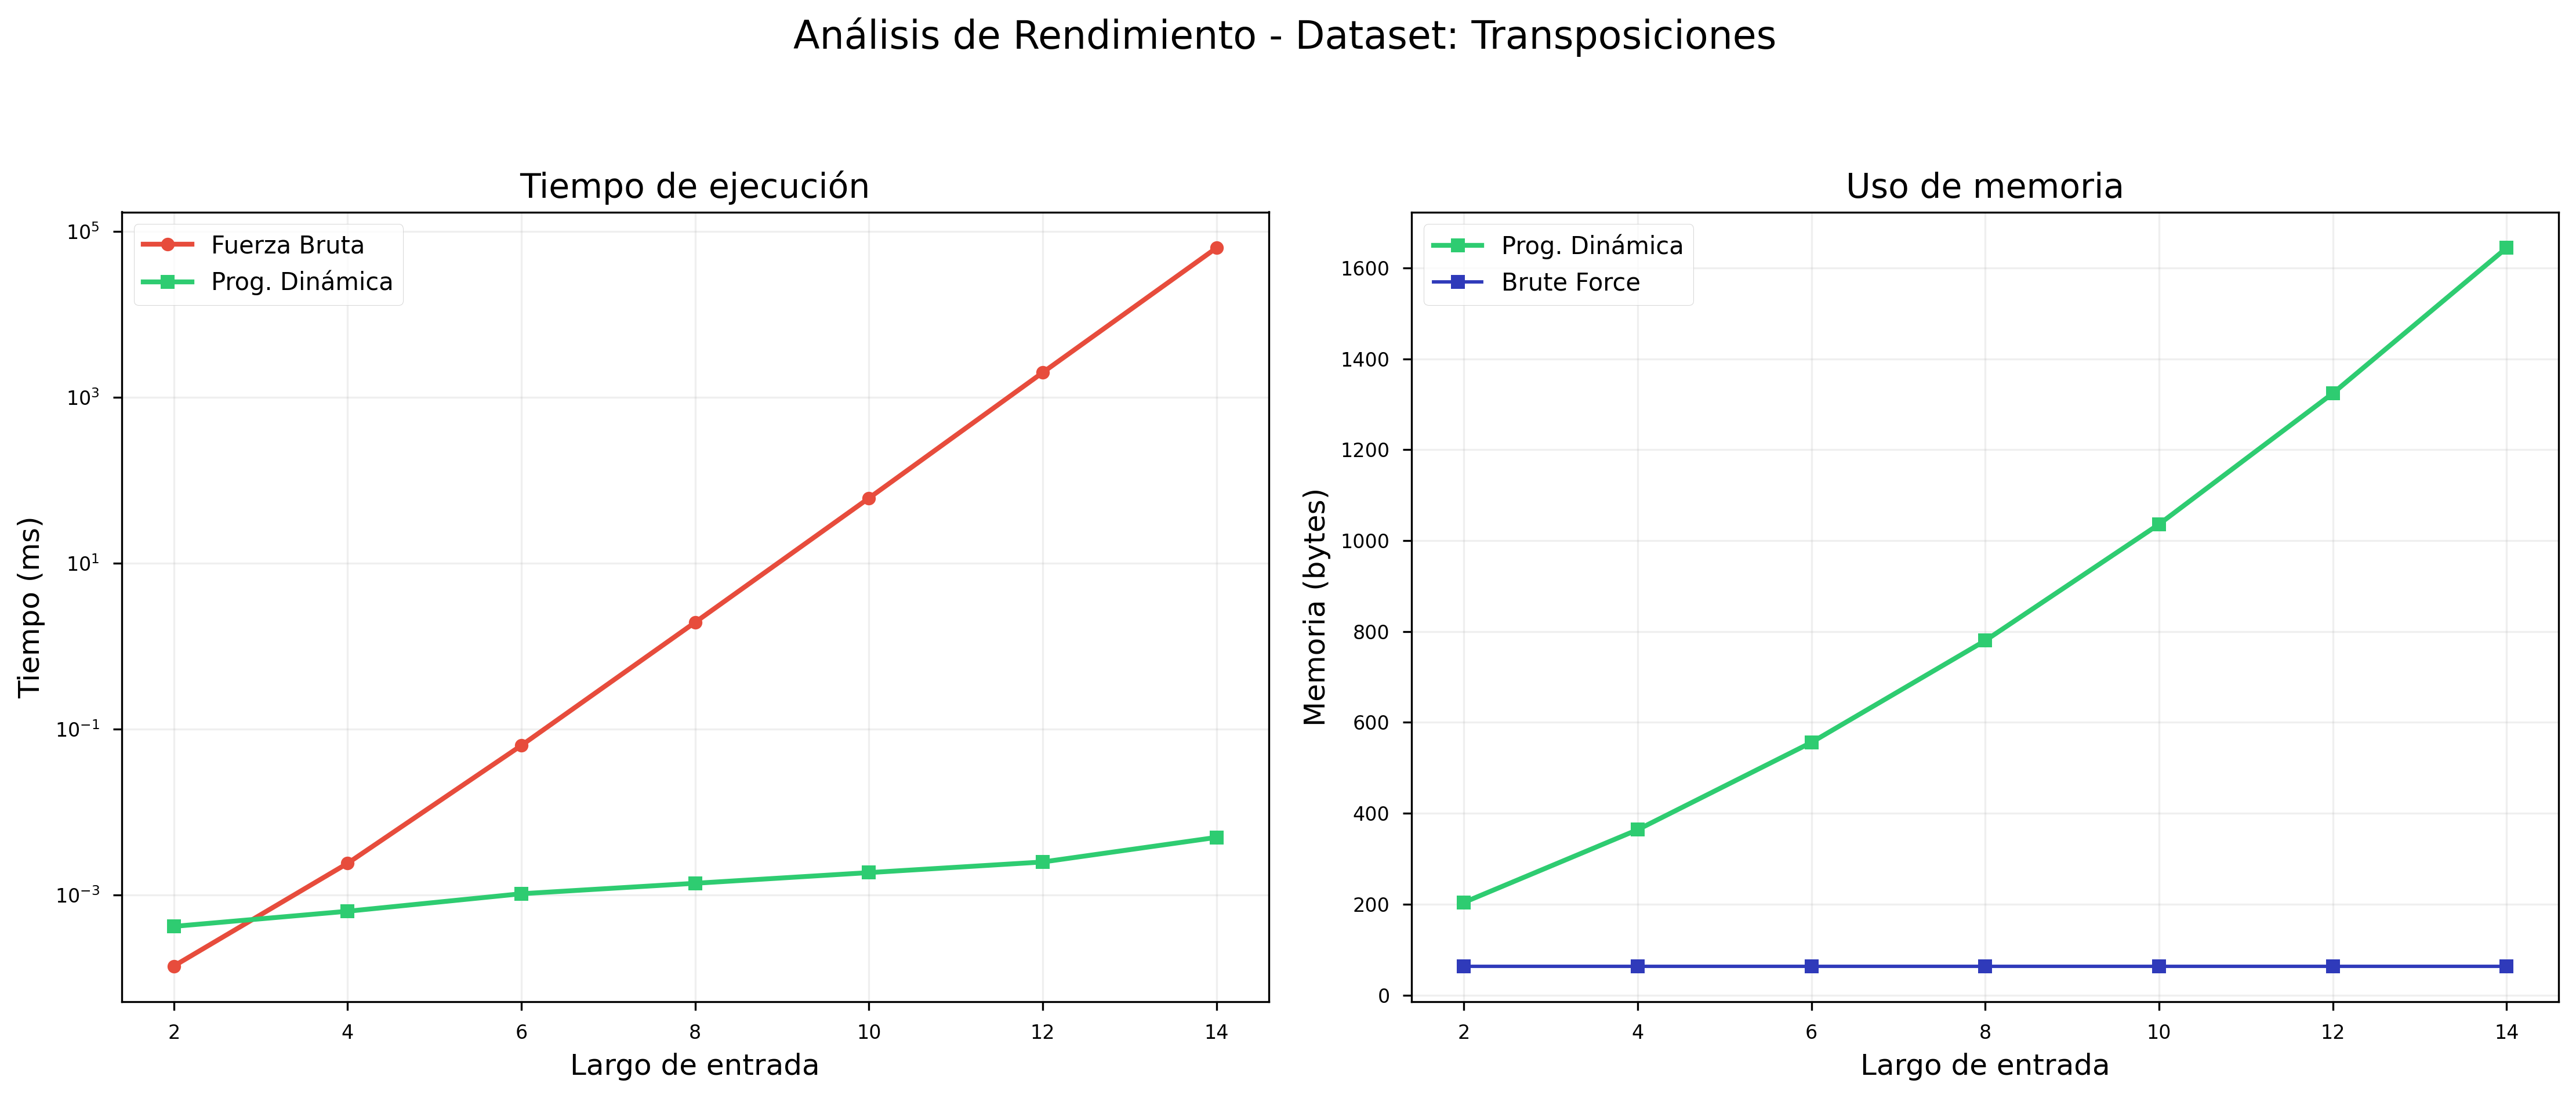
\includegraphics[width=\textwidth]{images/Transposiciones_analisis.png}
    \caption{Cadenas de pares transpuestos}
    \label{fig:scatterplot_2}
\end{figure}
\begin{figure}[H]
    \centering
    \begin{minipage}[t]{0.5\textwidth}
        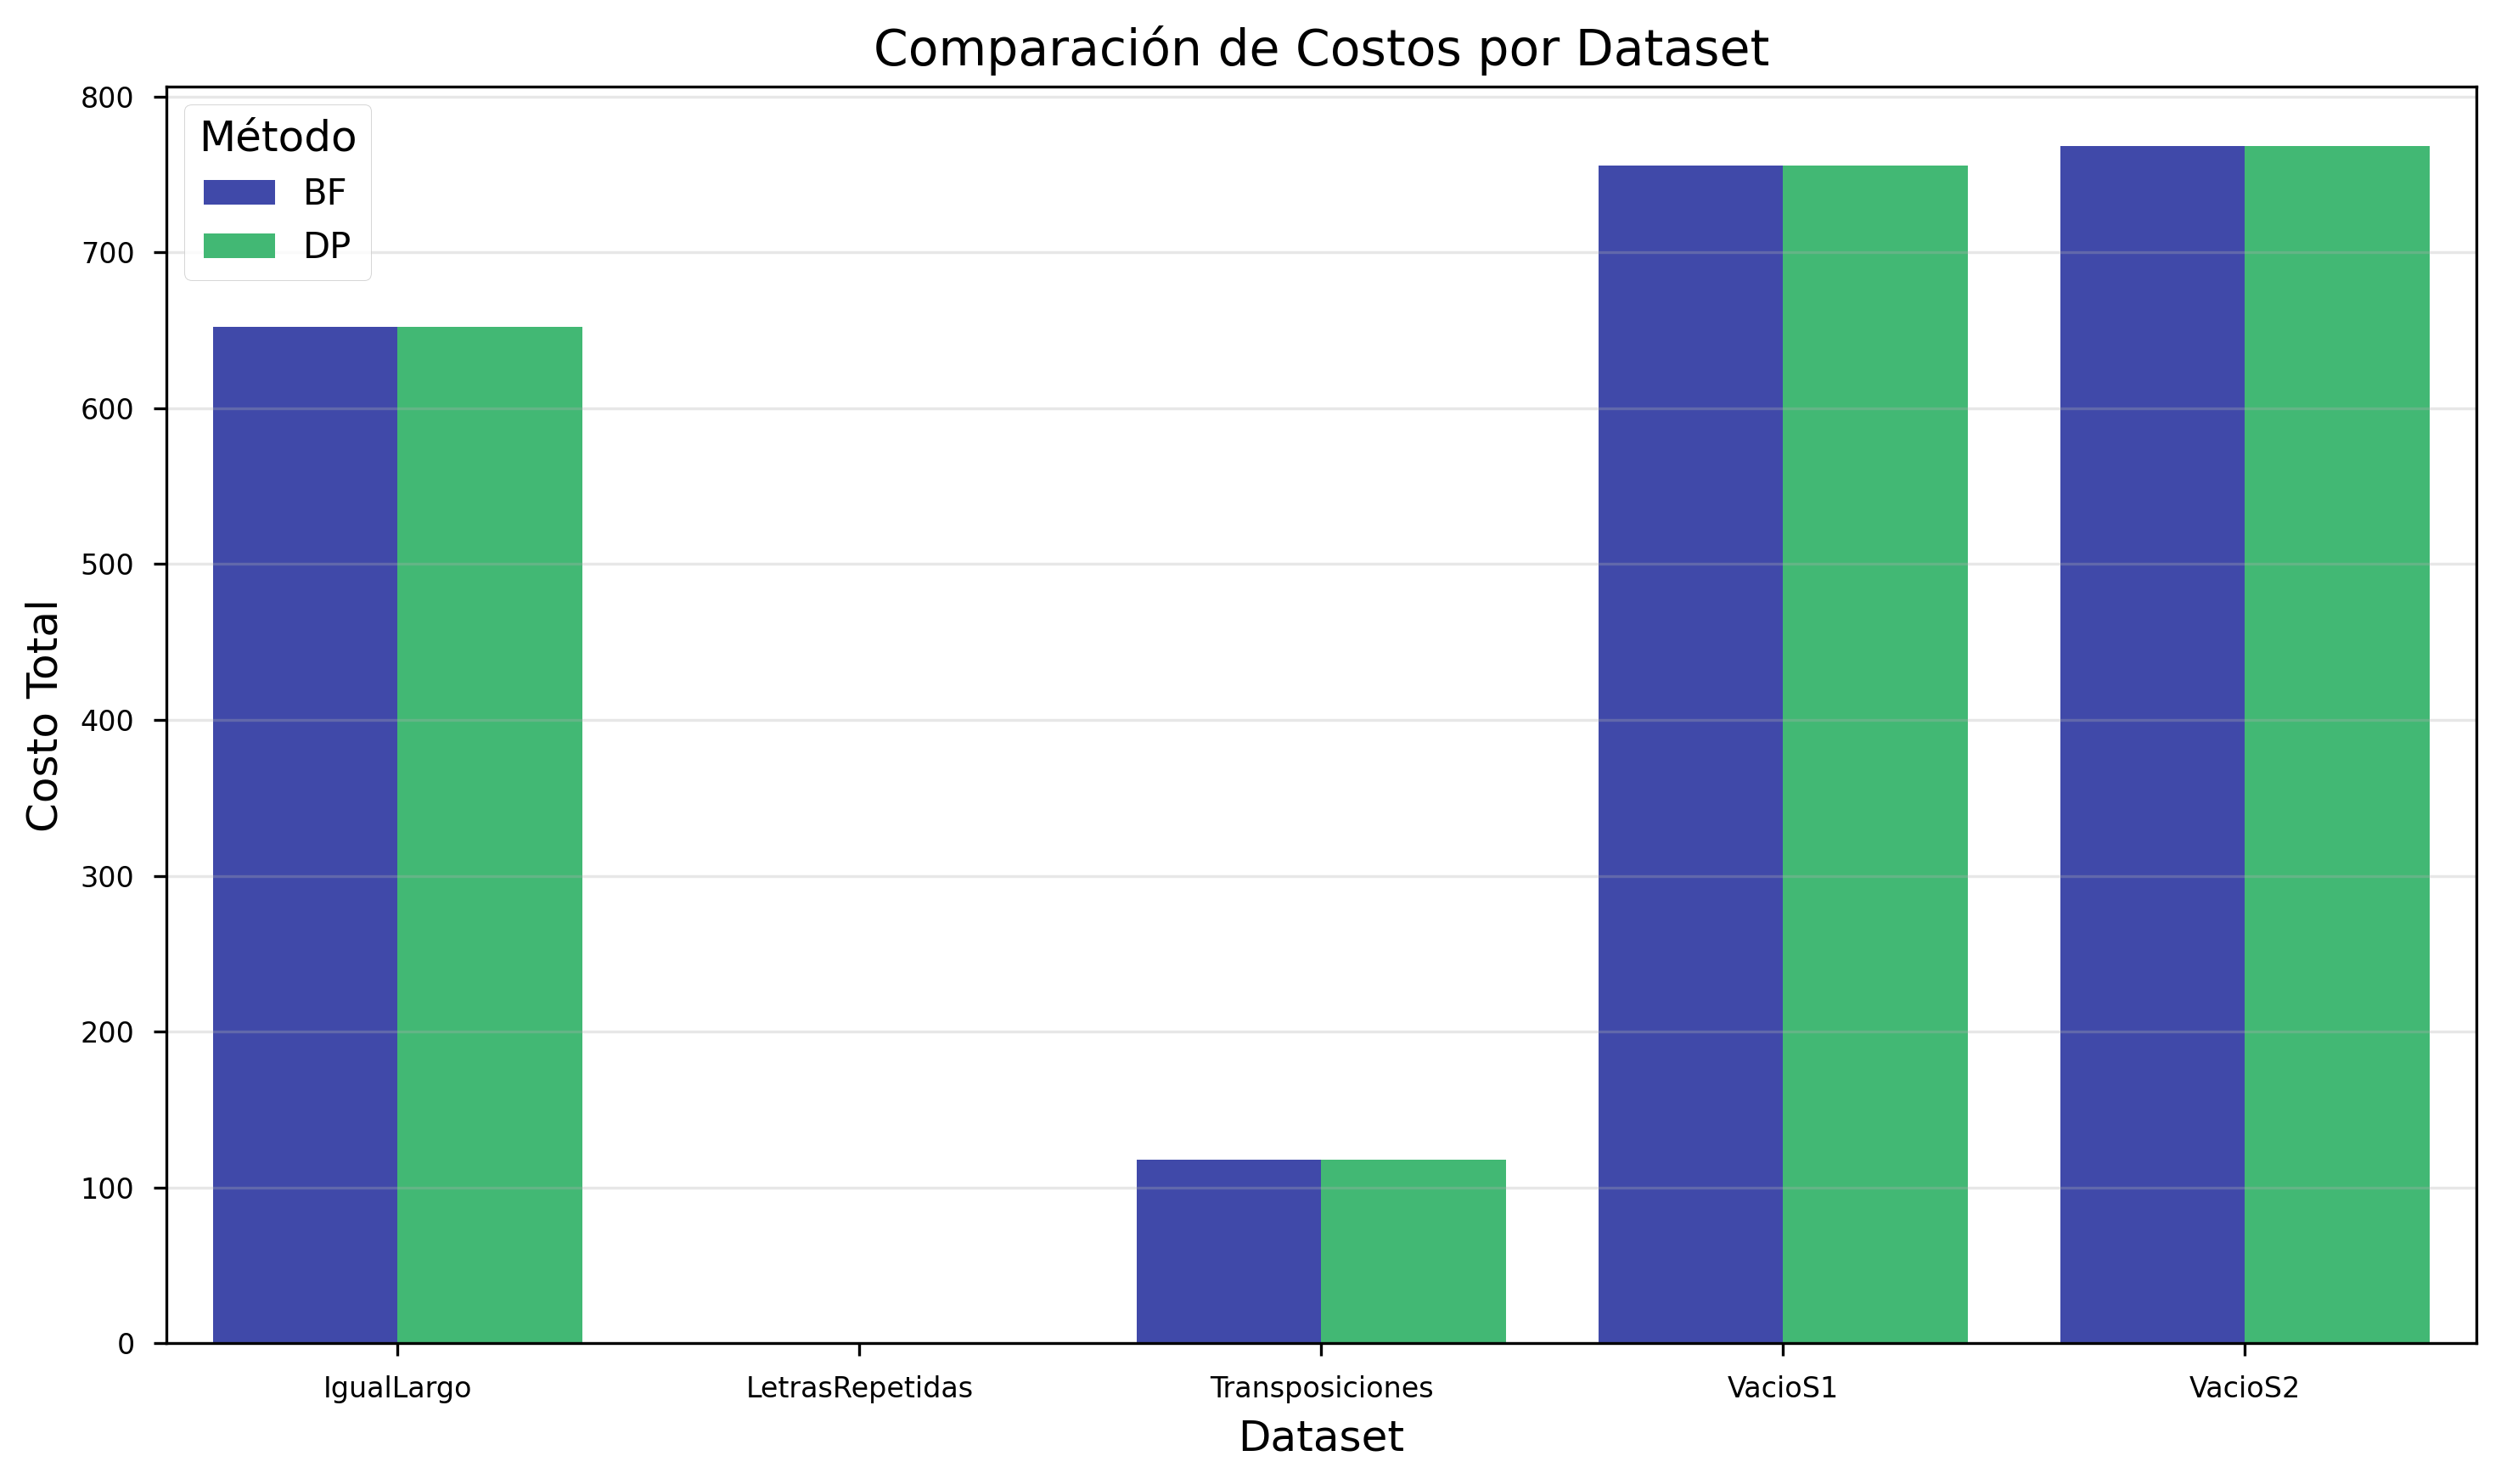
\includegraphics[width=\textwidth]{images/costos_por_dataset.png}
    \end{minipage}%
    \caption{Costos de edicion}
    \label{fig:barplot_1}
\end{figure}
Analizando las figuras 2 y 3 se puede observar que las transposiciones juegan un papel relevante dentro de este estudio,
puesto que si se busca disminuir el costo que toma editar 2 cadenas estas son una buena opcion a considerar, sin embargo, como ya se ha dicho
en la explicacion teorica, estas transposiciones incrementan la complejidad temporal del problema.  

\begin{figure}[H]
    \centering
        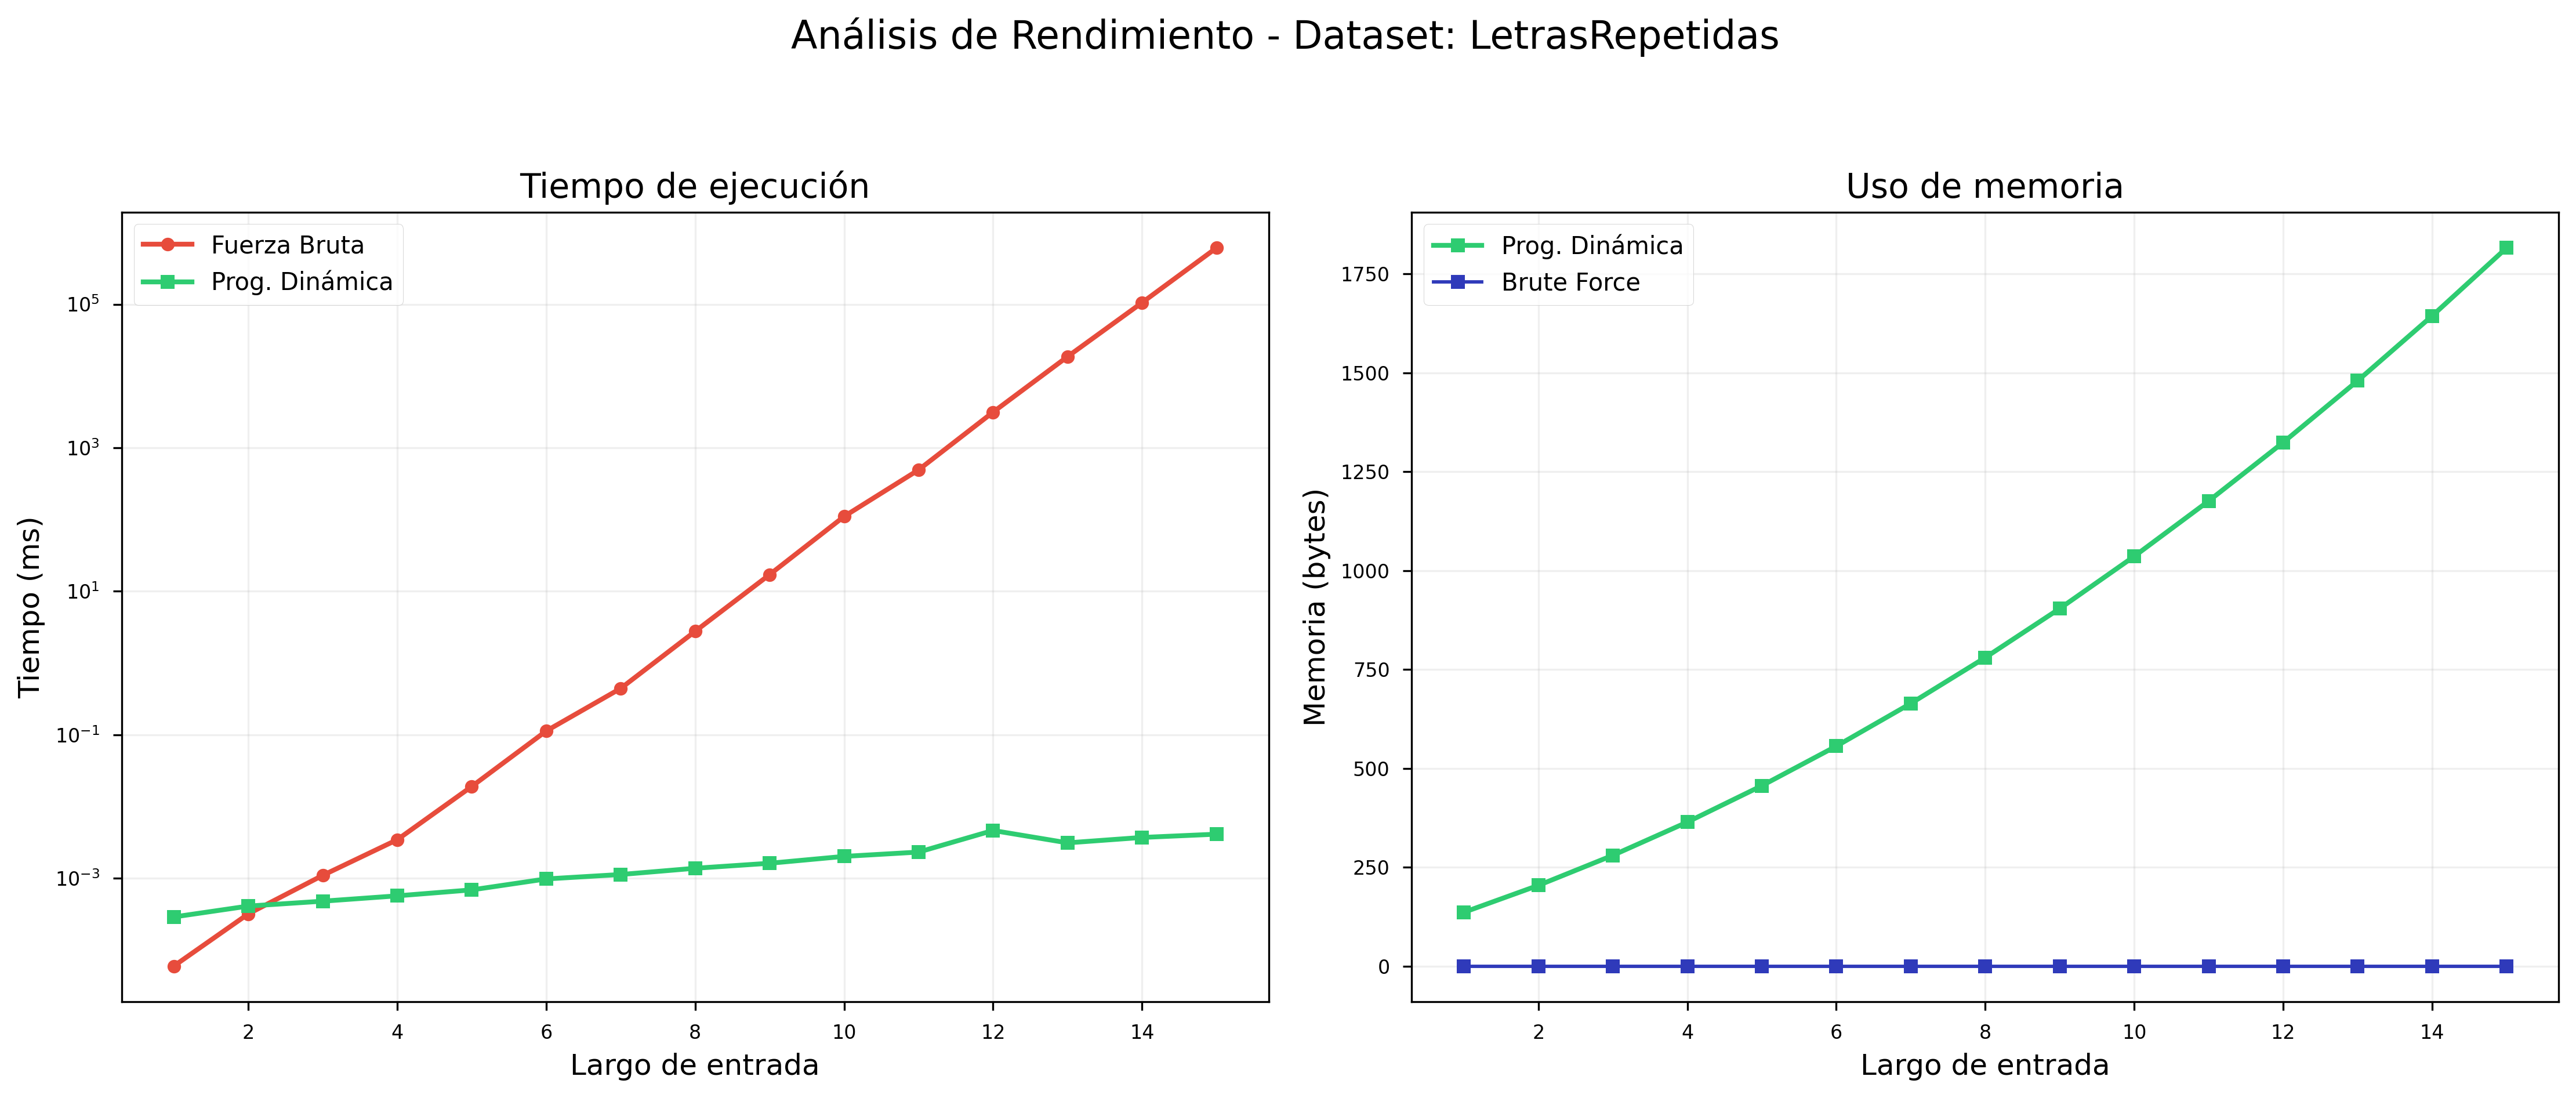
\includegraphics[width=\textwidth]{images/LetrasRepetidas_analisis.png}
    \caption{Cadenas de letras repetidas de largo creciente}
    \label{fig:scatterplot_4}
\end{figure}
La figura 4 se asemeja mucho a la figura 1, mas no son lo mismo, en la figura 4 se observa el peor caso posible para el caso de fuerza bruta, puesto
que todas las operaciones son realizables en todas las llamadas recursivas, por lo que la recursion alcanza una profundida mucho mayor que en cualquier otro
caso. Esto no solo afecta a fuerza bruta, puesto que en el enfoque de programacion dinamica tambien se debe relizar una mayor cantidad de operaciones a comparacion
de otros casos, pero debido a que cada operacion se ejecuta solo una vez para el par $(i,j)$ el tiempo de resolucion sigue siendo bajo

\begin{figure}[H]
    \centering
        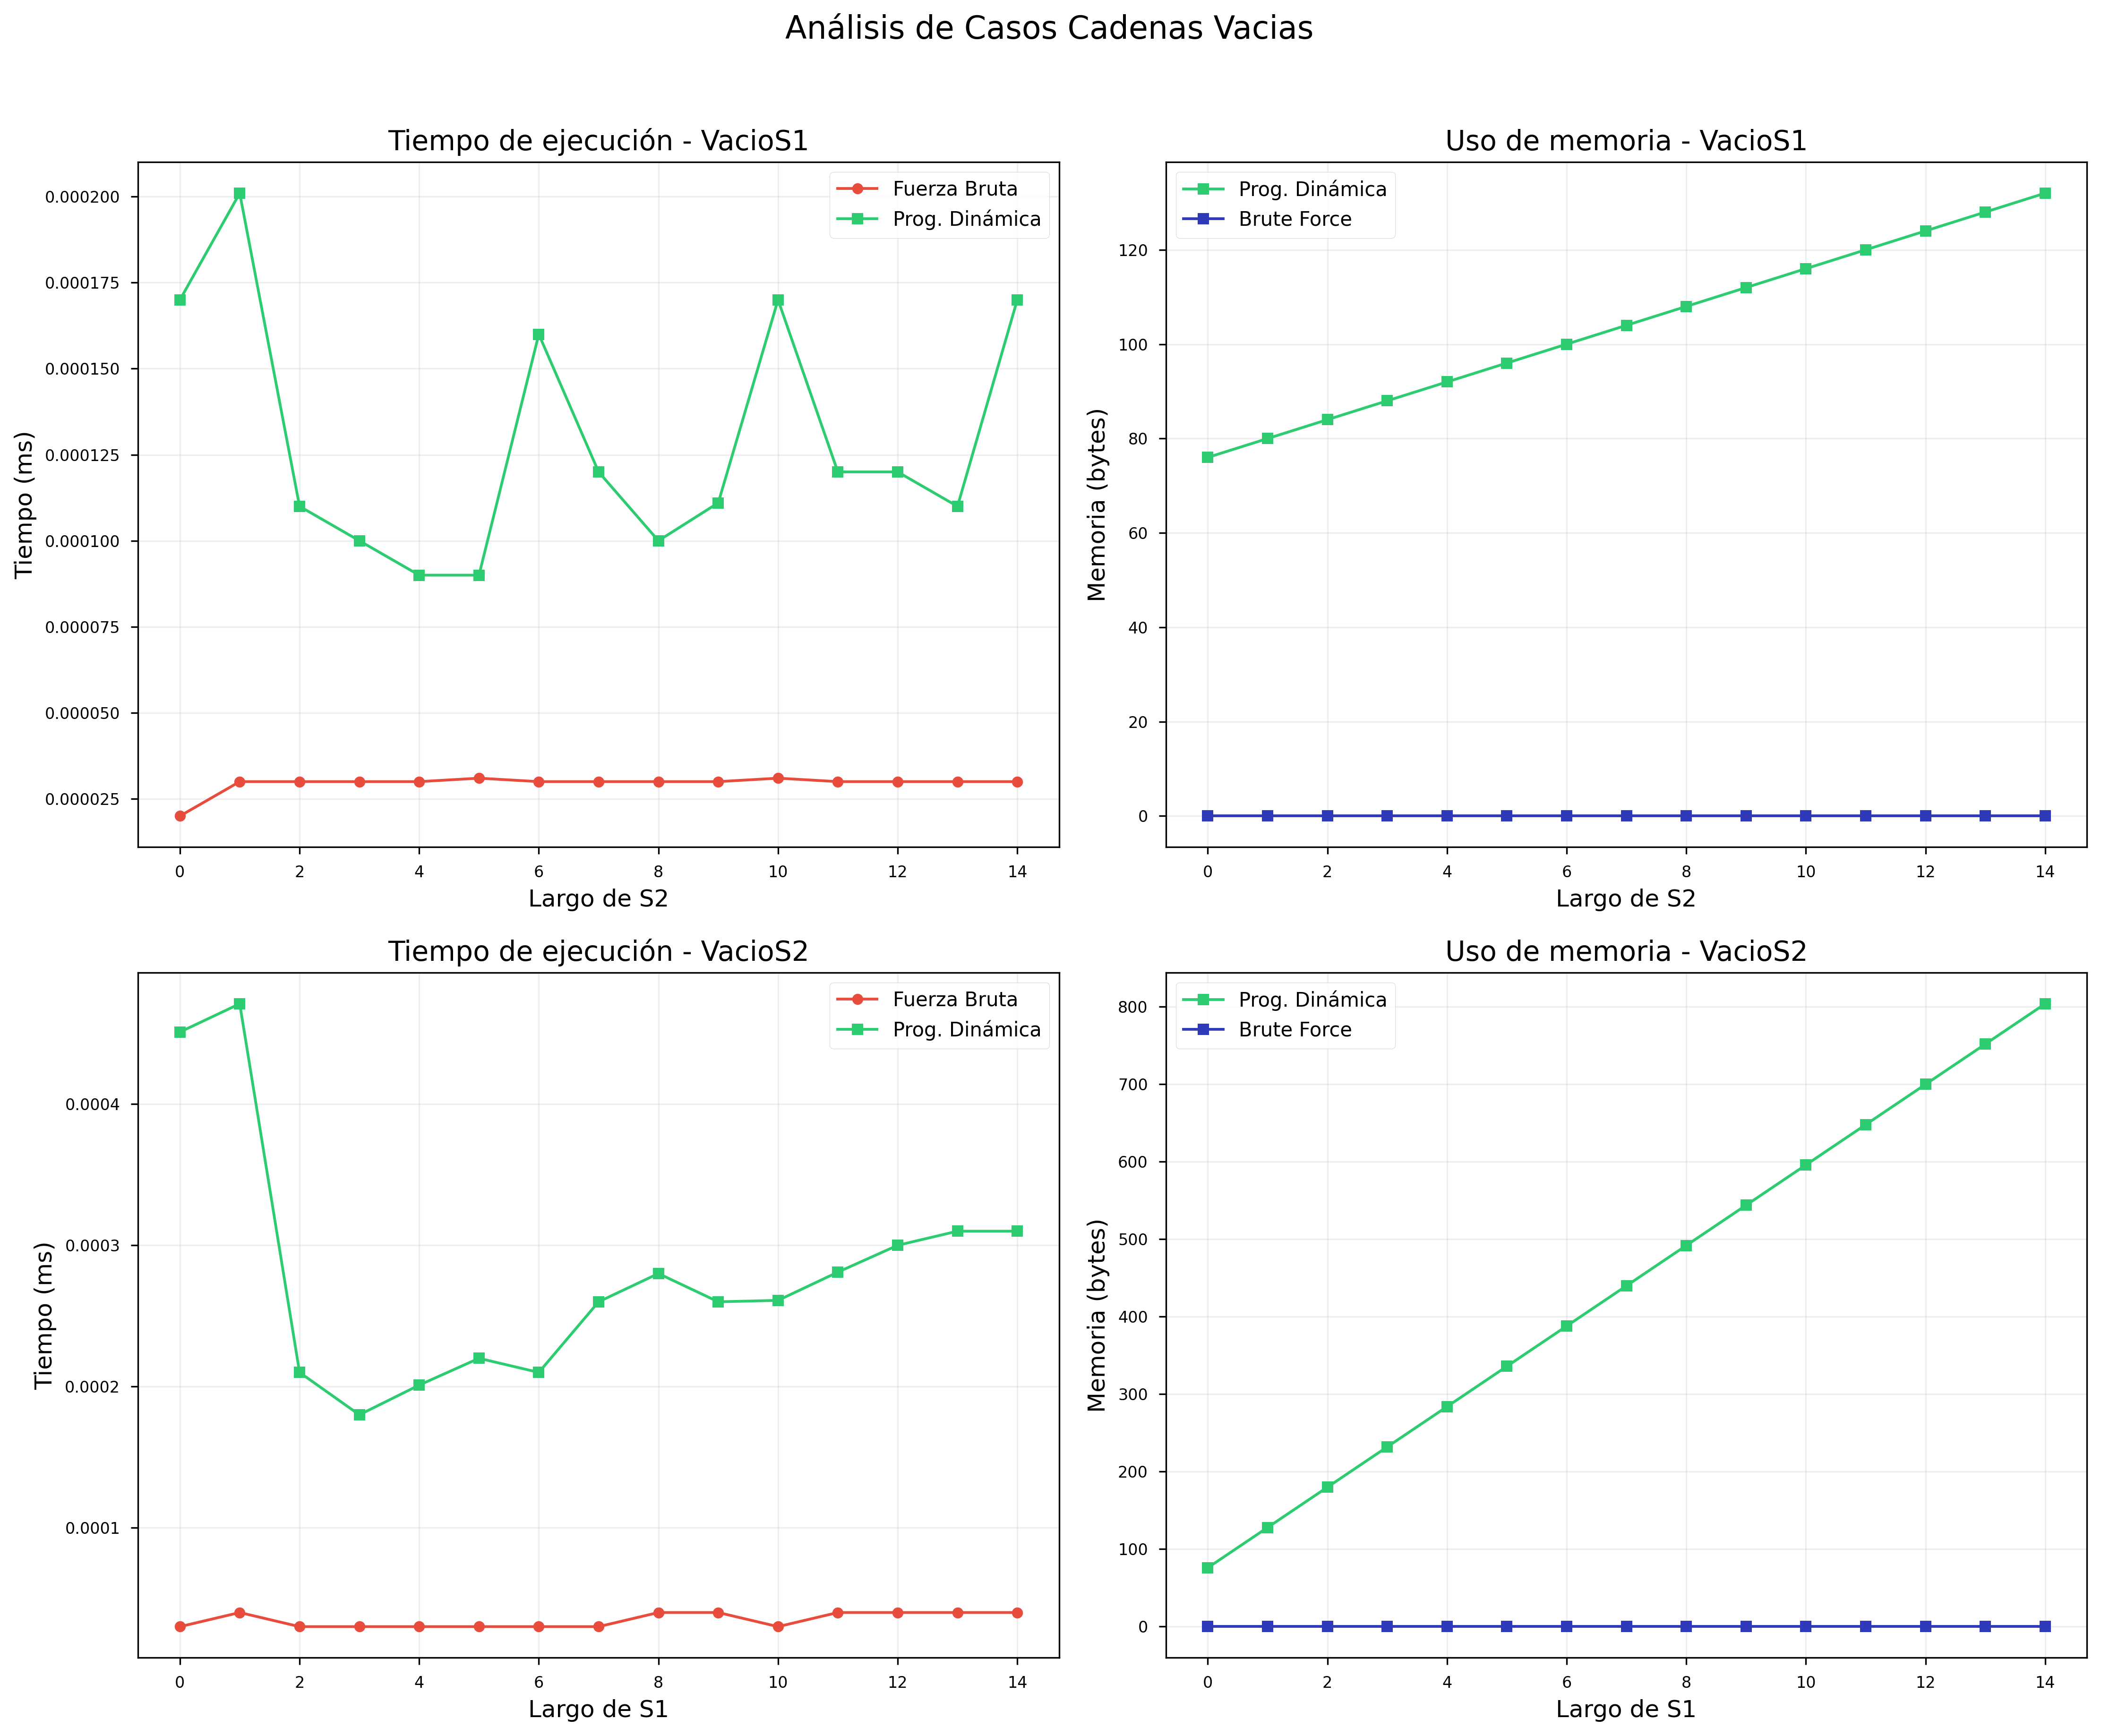
\includegraphics[width=\textwidth]{images/casos_especiales.png} 
        \caption{Casos Cadenas Vacias}
    \label{fig:scatterplot_5}
\end{figure}
En la figura 5, en contraste a la figura 4, se puede observar el mejor caso posible para fuerza bruta, puesto que no todas las operaciones son relizables, sino solamente
inserciones o eliminaciones constantes y no llega nunca a ser exponencial, en contraste tenemos al enfoque de programacion dinamica, el cual se demora más
debido al uso de una matriz de cache, la cual se debe inicializar y posteriormente resolver el problema.
\begin{figure}[H]
    \centering
        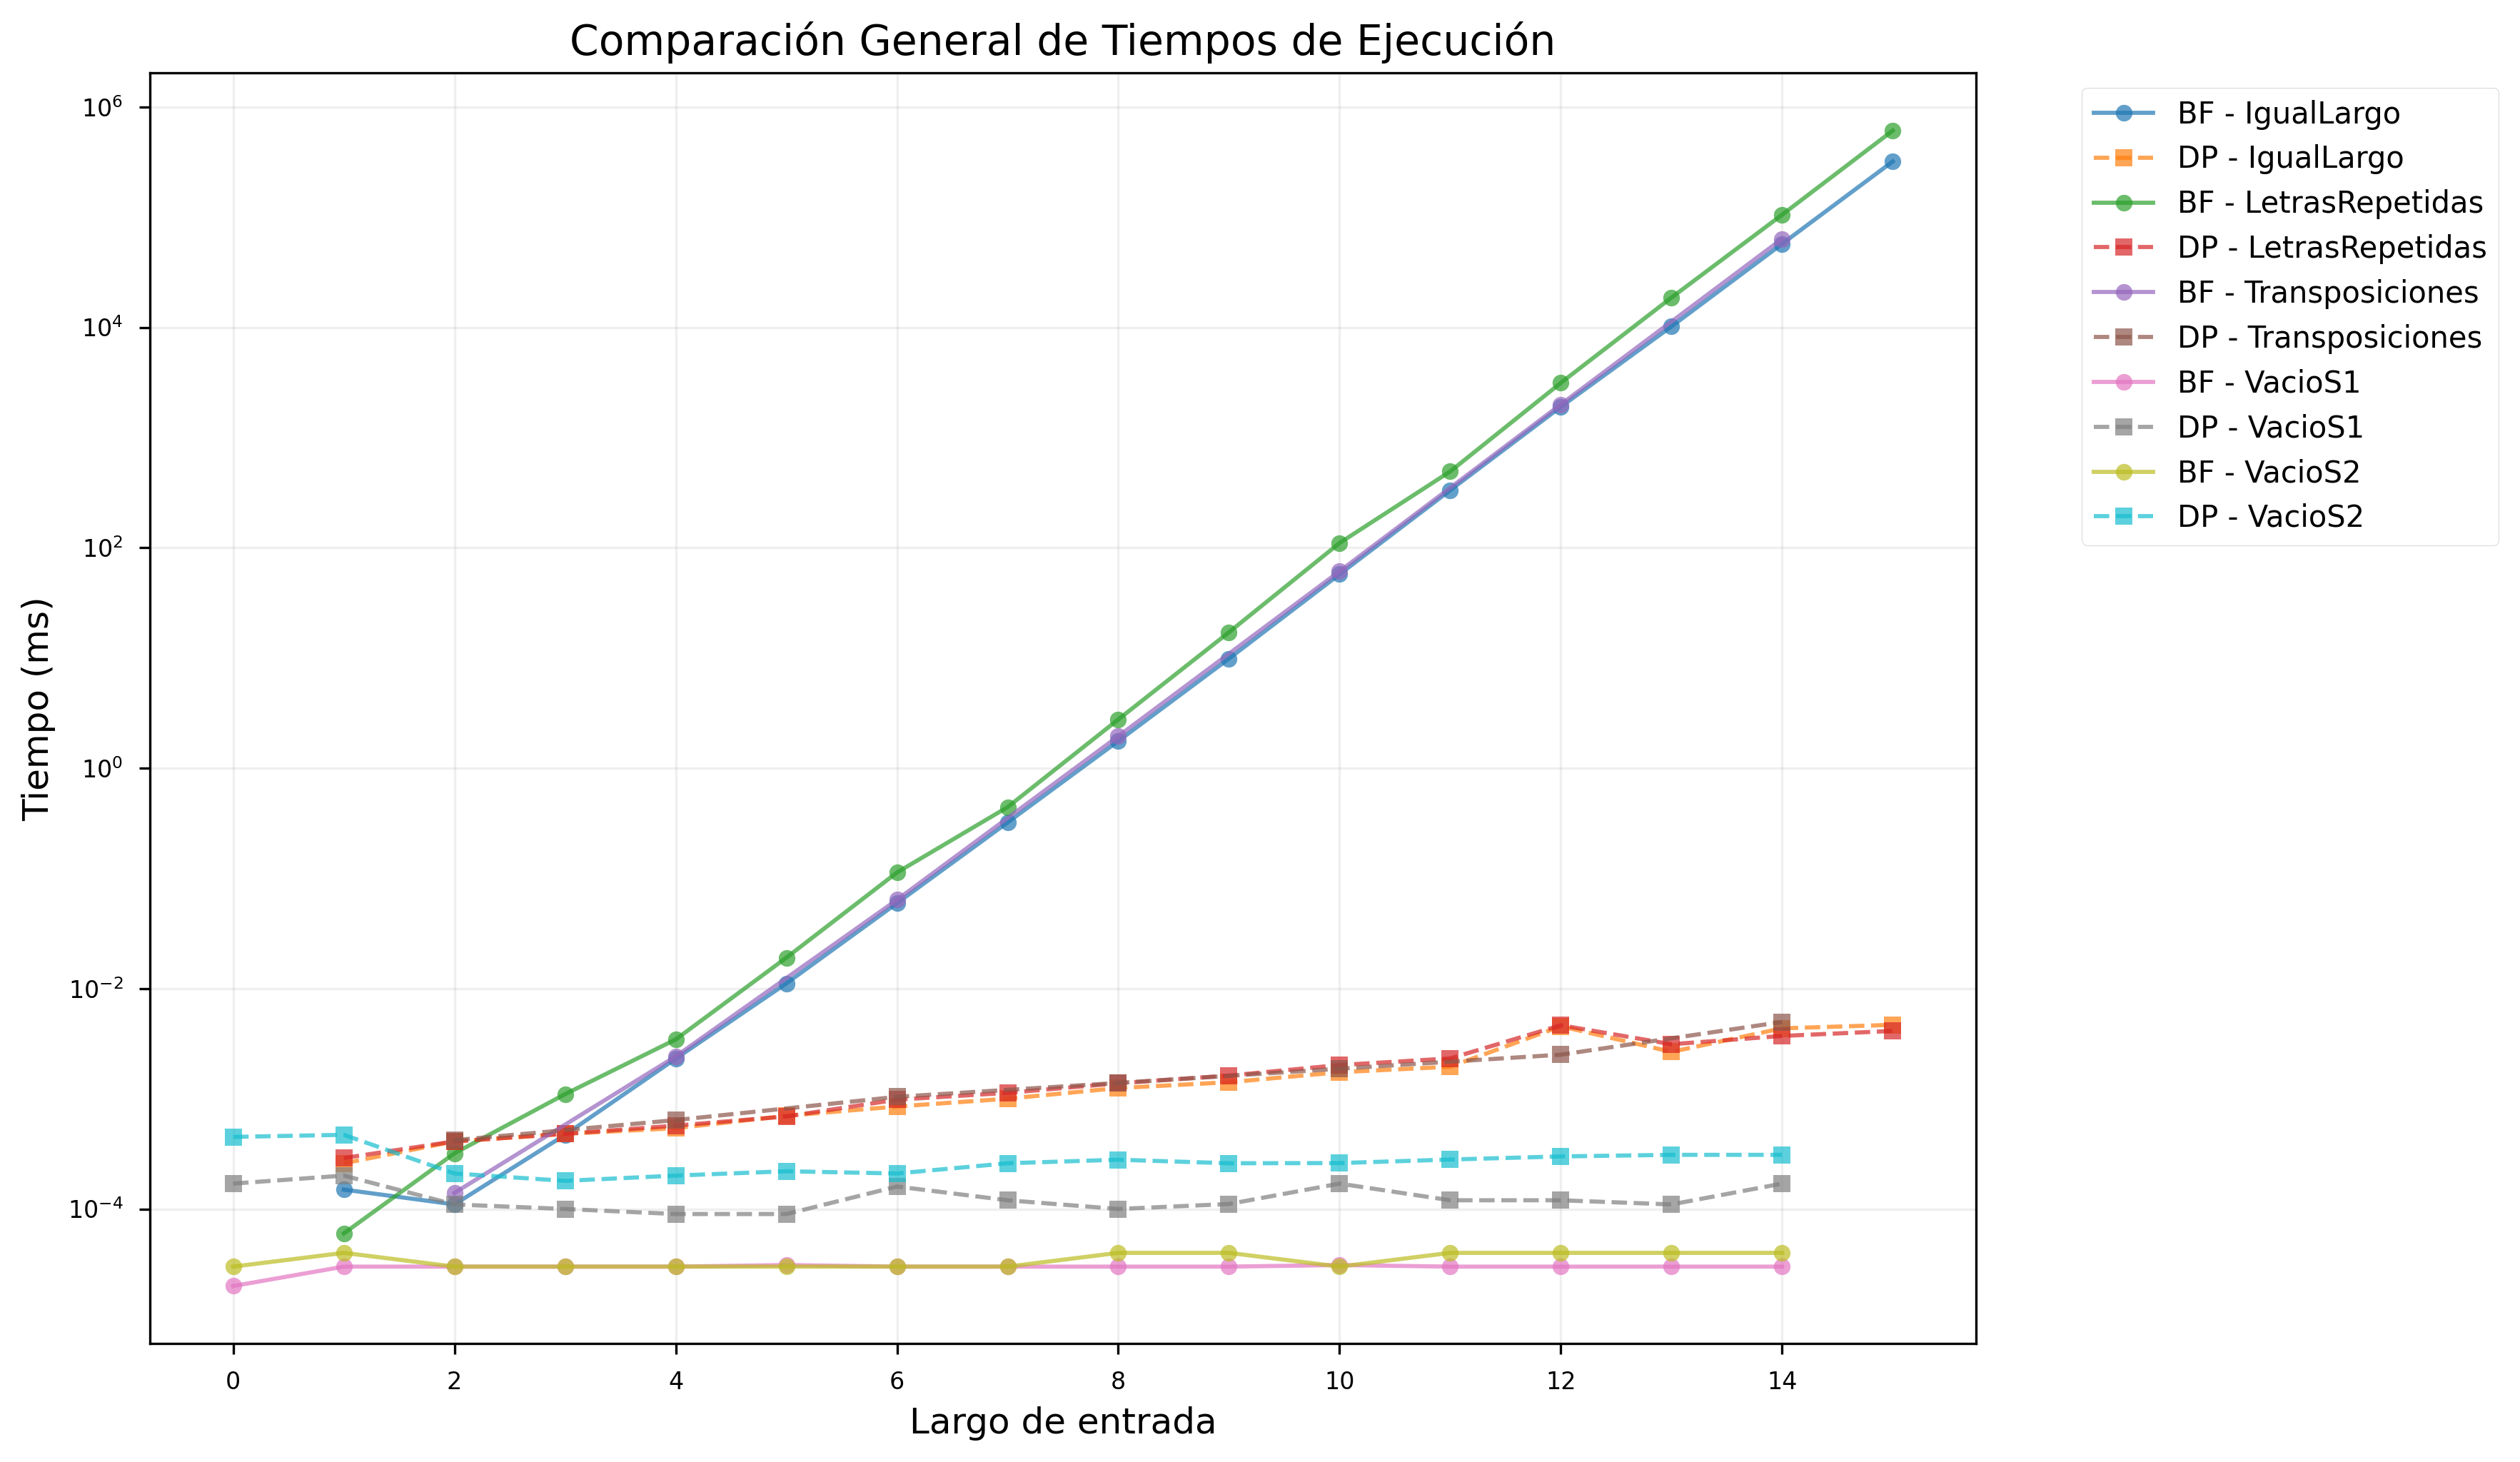
\includegraphics[width=\textwidth]{images/comparacion_general_tiempos.png}    
    \caption{Resumen general de resultados}
    \label{fig:scatterplot_6}
\end{figure}
En la figura 6 se observa un resumen general de todos los casos anteriores, del cual se extrae que si queremos resolver el problema de la menor distancia 
es importante tener en cuenta que el enfoque de fuerza bruta para cadenas vacias puede llegar a ser util, sin embargo el enfoque de 
programacion dinamica es una buena opcion general.
